%% \chapter[htoc-titlei][hhead-titlei]{htitlei}
%% -----------------------------------------------------------------------------
\chapter[The Large Hadron Collider and the ATLAS Experiment][The Large Hadron Collider and the ATLAS Experiment]{The Large Hadron Collider and the ATLAS Experiment}
\label{chapter:lhc}
%test
\section{The Large Hadron Collider}


Production of a sufficient number of high energy collisions to adequately explore
the physics of electro-weak symmetry breaking required the development of one
of the most complex machines ever built, the Large Hadron Collider or LHC. 

The LHC is the world's highest energy particle accelerator 
and is located 100m underneath the French-Swiss border at the European Organization
for Nuclear Research (CERN) in a 26.7 km tunnel. The technology involved in the development of the LHC is an enormous achievement
it its own right and is documented in detail here \cite{1748-0221-3-08-S08001,Pettersson:291782,Linnecar:1176380}. 
The LHC is a circular machine capable of accelerating beams of protons and colliding them at center of mass 
energies up to $\sqrt{s} = 14$ TeV at 4 collision sites around the ring, where 4 experiments
are housed (ATLAS\cite{ATLAS_detector}, CMS\cite{1748-0221-3-08-S08004}, LHCb\cite{1748-0221-3-08-S08005}, and ALICE\cite{1748-0221-3-08-S08002}). Figure \ref{figure:lhc_lhc} is a diagram
of the layout of the LHC and its experiments\cite{Team:40525}. The LHC also operates in a mode with beams of 
heavy ions. The LHC is composed of thousands of super-conducting Niobium-Titantium 
magnets, cooled to 1.9 K with liquid Helium, which steer and focus the 
particle beams, and superconducting resonant-frequency (RF) cavities, which boost the beam
to higher energies. 

% magnets
\begin{figure}[!t]
\centering 
\includegraphics[width=0.75\textwidth]{figs/lhc/lhc.pdf}
\caption{ Diagram of the Large Hadron collider and location of the 4 main experiments (ATLAS, CMS, LHCb, and ALICE) around
  the ring. The diagram also shows the location of the SPS, the final booster ring in the accelerator complex that accelerates
    the protons to 450 GeV before injection into the LHC. 
}
\label{figure:lhc_lhc}
\end{figure}



\subsection{The Accelerator Complex}

The accelerator complex is a progressive series of machines with the LHC as the final stage.
Protons are obtained from hydrogen atoms and are accelerated to 50 MeV using the
Linac2, a linear accelerator, before being injected into the Proton-Synchrotron Booster (PSB). In
the PSB the protons are accelerated to energies of 1.4 GeV for injection
in to the Proton-Synchrotron (PS). The PS accelerates the protons to 25 GeV
and dumps bunches into the Super Proton Synchrotron (SPS), where they 
are accelerated to 450 GeV and finally dumped into the LHC for full acceleration. The PS and SPS are circular accelerators
that were important in past physics discoveries and have been re-purposed for use in the LHC complex. 

\subsection{Beam Parameters and Collisions} 

For the physics studied at the ATLAS experiment, the two most important parameters of
the collisions are the center of mass energy (CME)  and instantaneous luminosity ($\mathcal{L}$).
High center of mass energies are necessary for the production
of new high mass particles, and, because the constituents of the actual collisions
are the partons of the proton, the CME of the collisions must in general
be much higher than the mass of the particles produced. 

The instantaneous luminosity of the collisions is a measure of the
collision rate. The integrated luminosity over time is a measure of the size
of the dataset and when multiplied by the cross-section of a particular process
gives the total number of expected events produced for that process.
Instantaneous luminosity depends on the number of colliding bunches of protons,
the intensity of those bunches, the revolution
frequency, and the normalized transverse spread of the beam in momentum and position
phase space, called the emittance, and the transverse beam size. The LHC has the
option for colliding beams with 2808 bunches of protons, each with around $10^{11}$ protons,
at a rate of one bunch collision every 25 ns, or 40 MHz. These parameters correspond
to a design luminosity of around $10^{34}$ cm$^{2}$ s$^{-1}$ or 10 nb$^{-1}$ s$^{-1}$,
equivalent to 1 Higgs every 5 seconds. For various reasons, the bunch collision
rate was help at 20 MHz for the 2011 and 2012 runs. 

\section{The ATLAS Experiment}

This section provides a brief overview of the ATLAS experiment. The ATLAS detector
is centered on one of the LHC collisions points, located 100 m underground. Through
the combination of a number of subsystems, it is designed to identify the 
particles arising from these collisions, measure the energy and momentum  
of these particles, and make fast decisions about the content
of each collision, in order to save a small fraction of measured collision events
for offline study. 

ATLAS, shown in Figure~\ref{figure:lhc_atlas},  possesses cylindrical symmetry around the beam pipe. It weighs 7000 tons,
has a diameter of roughly 25 m and length of 46 m. ATLAS was designed to be a multi-purpose
hermetic, particle detector, able to identify many types of particles, and designed to provide
a snapshot of the entire collision event. The detector sub-systems form concentric rings 
around the beam-line at increasing distance. From closest to the beam outward, they are:

\begin{itemize}

\item \textbf{Inner Detector:} The inner detector (ID)\cite{IDTDR1,IDTDR2} is immersed in a solenoidal magnetic field\cite{MagnetTDR} and provides measurements of charge particle tracks, through three subsystems: the Pixel Detector\cite{PixelTDR,PixelSensor}, the Semi-Conductor Tracker (SCT)\cite{SCTBarrel,SCTEndcap}, and Transition Radiation Tracker(TRT) \cite{TRTStraws, TRTBarrel,trtelec}. 

\item \textbf{Calorimeter:} The calorimeters measure the energy of particles that participate in the electromagnetic (photons, electrons) and hadronic interactions (pions, protons, neutrons, etc.), by forcing them to shower in dense material. The hermeticity of the calorimeters allows for missing transverse energy measurements. The calorimeter is composed of the liquid argon electromagnetic calorimeter (LAr)\cite{LArTDR:1996fq}, the hadronic tile calorimeter\cite{TileTDR}, the liquid argon hadronic endcap calorimeter, and the forward calorimeters.

\item \textbf{Muon Spectrometer:} The muon spectrometer (MS) sub-systems\cite{MuonTDR} form the outermost detector systems and measure the momentum of minimum ionizing muon tracks, as all other particles are stopped by the calorimeters. The muon systems are immersed in a toroidal magnetic field \cite{MagnetTDR} and are composed of 4 different sub-systems for triggering and tracking measurements \cite{RPCPaper,MDTPaper,CSCPaper}. 

\item \textbf{Triggering Systems:}  The trigger and data acquisition systems\cite{L1TDR,HLTTDR} read out data from the detector through a three-tiered hardware and software decision making framework to record the most interesting physical processes for a broad physics analysis program.   

\end{itemize}


These systems are discussed in depth in the following sections.
\begin{figure}[!t]
\centering 
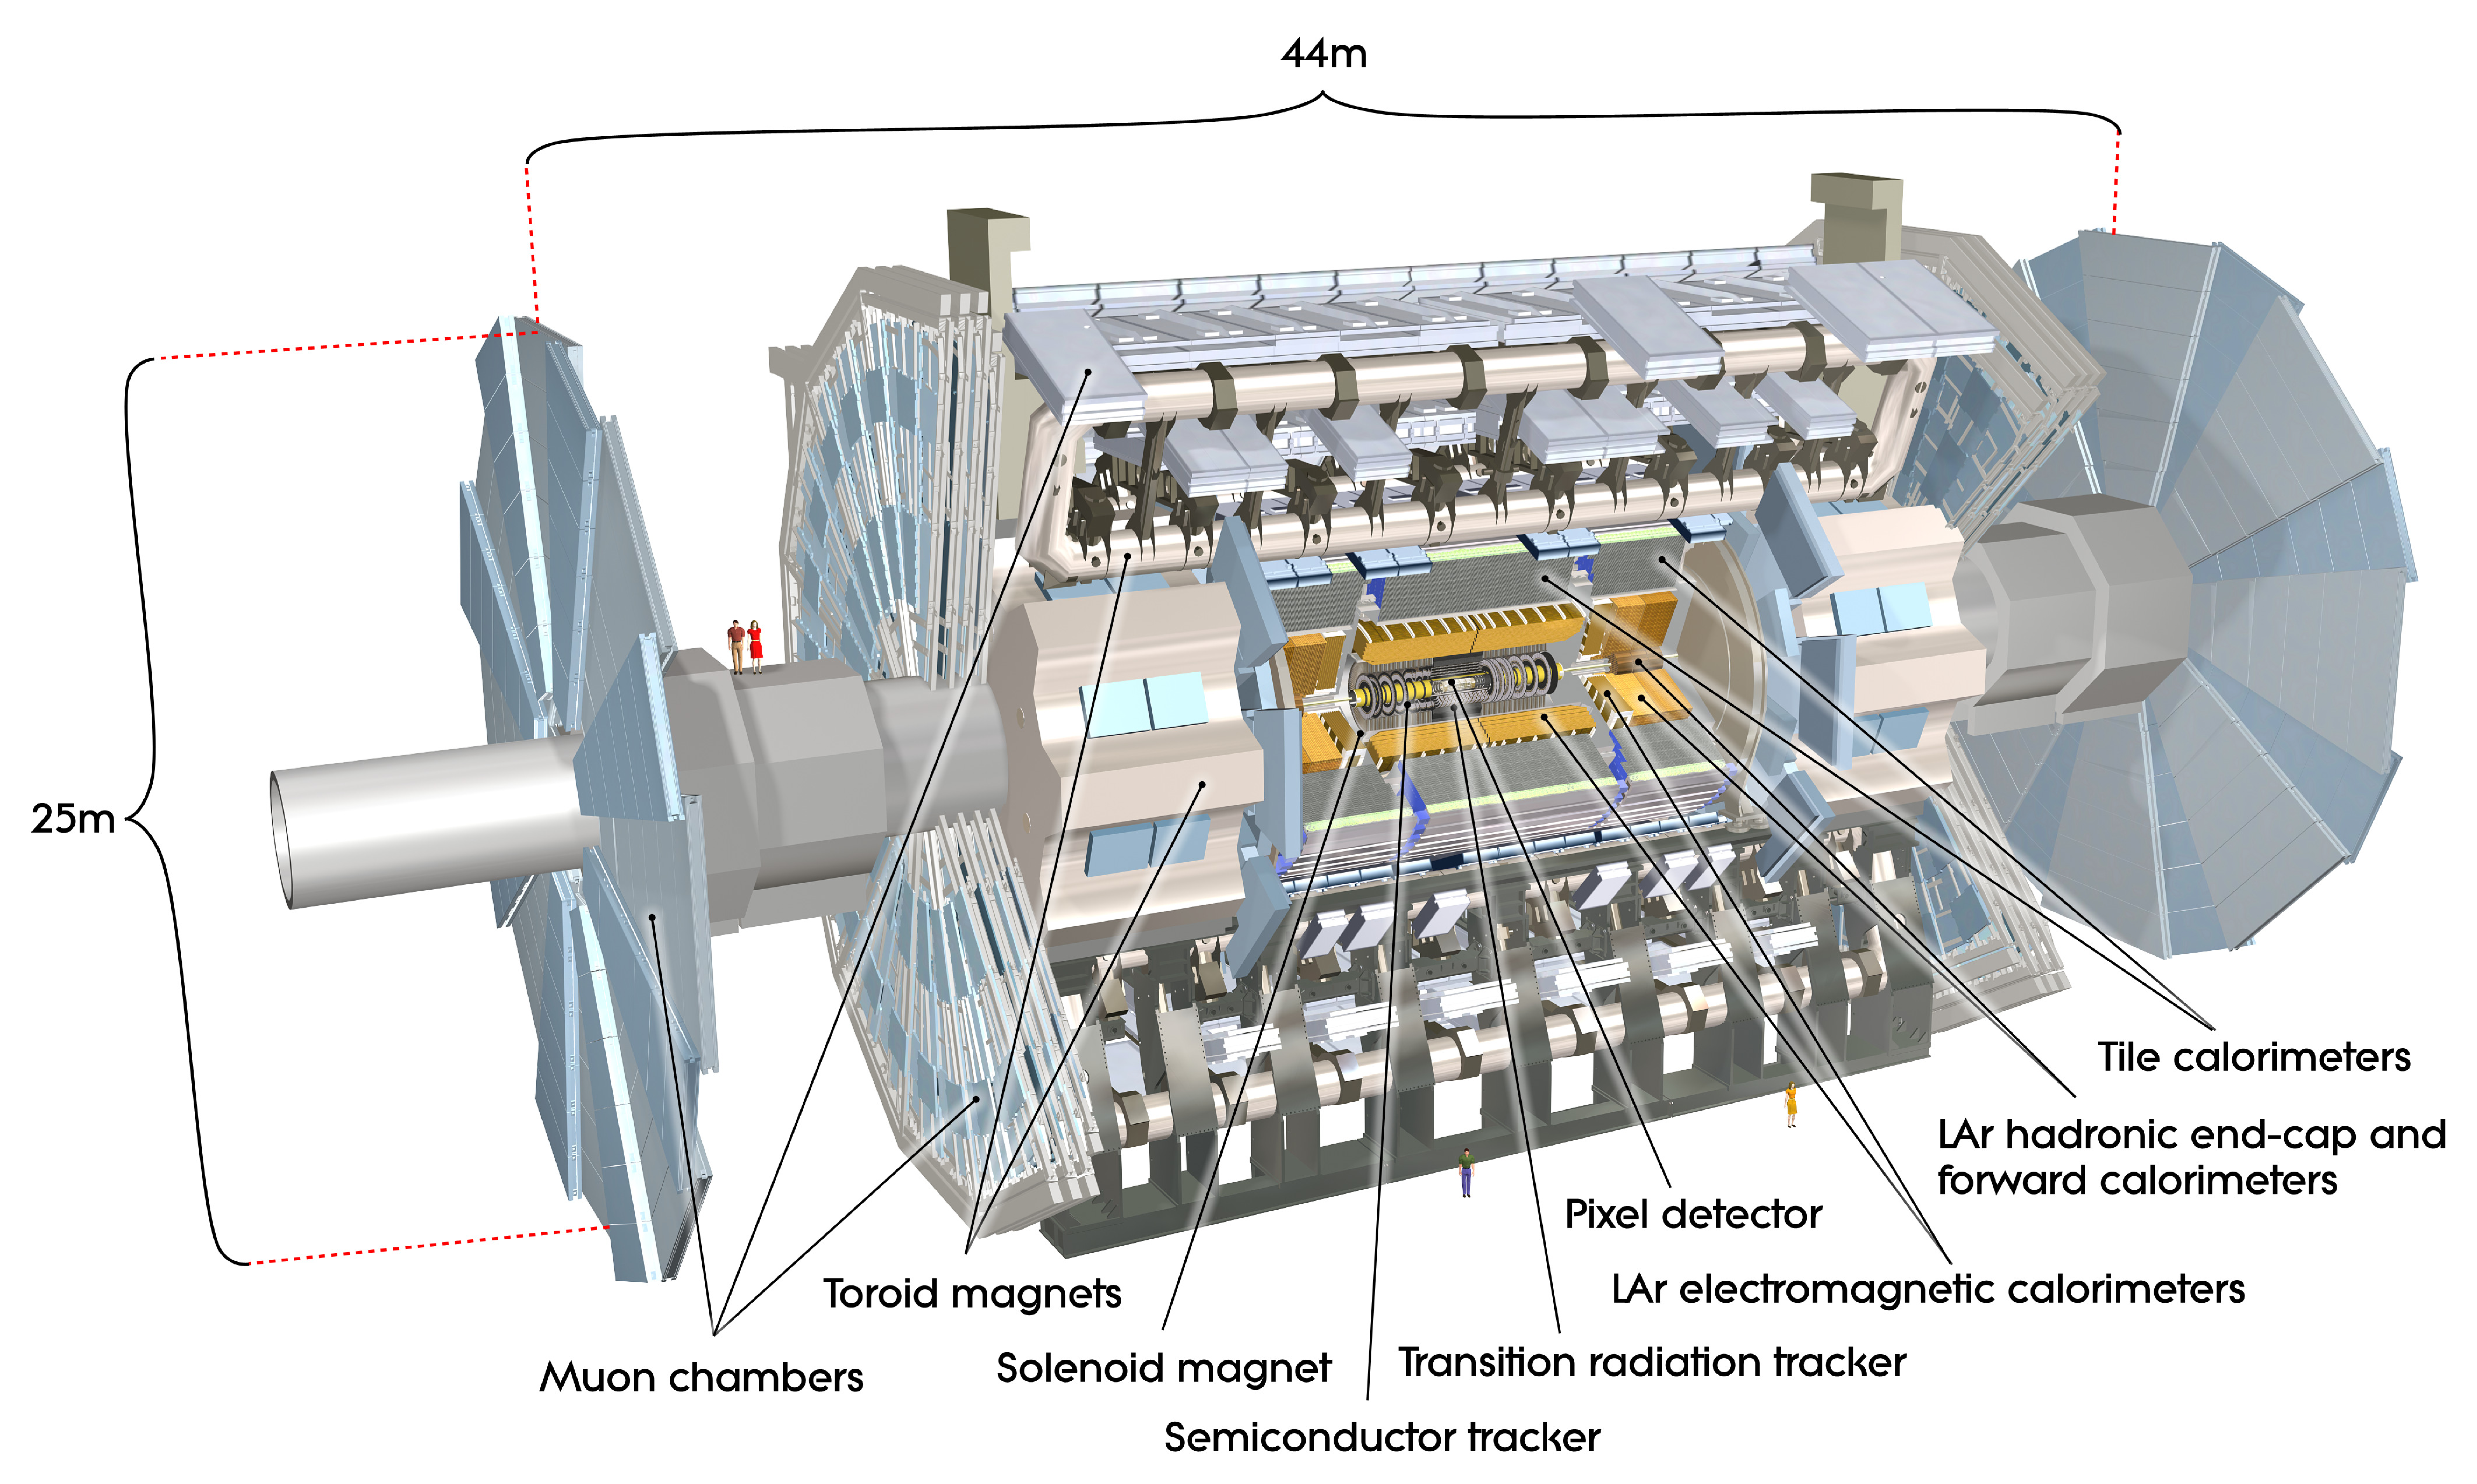
\includegraphics[width=0.9\textwidth]{figs/lhc/ATLAS-eps-converted-to.pdf}
\caption{ Diagram of the ATLAS detector and subsystems 
}
\label{figure:lhc_atlas}
\end{figure}


\subsection{Detector Coordinate System}

ATLAS uses a right-handed  coordinate system centered at the nominal proton interaction point. The beam line defines the $z$-axis. The $x-y$ plane is perpendicular to the beam line and is referred to as the transverse plane. The transverse plane holds special significance in reporting measurements, because the initial momentum of the hard collision system is 0 along the transverse plane in the laboratory rest frame. Particle momenta measured along the transverse plane is called transverse momenta, and labeled $p_T$.  The momentum of the colliding proton-proton system is also 0 along the $z$-axis but the colliding partons may have vastly different momenta. Thus, momentum of the hard colliding system along the $z$-axis differs collision to collision. 

Because ATLAS possesses a rough cylindrical symmetry, cylindrical and polar coordinates are used to describe particle trajectories and detector positions. The radial coordinate, $R$, describes transverse distances from the beam line. An azimuthal angle, $\phi$, describes angles around the $z$-axis, and a polar coordinate, $\theta$, describes angles away from the $z$-axis. The polar angle is often expressed in terms of pseudo-rapidity, defined as $\eta=-$ln(tan($\theta/2$)). Distances in $\eta-\phi$ space are often used to describe the proximity of objects in the detector, $\Delta R = \sqrt{\eta^2 + \phi^2}$.

The `barrel' and `endcap' are classifications that are used to label the position of sub-detectors. Barrel sub-detectors occupy positions more central to the detector at $|\eta|$ values roughly less than 1-2, while the endcap calorimeters extend farther in $|\eta|$. The barrel-endcap transition region contains detector services. Also, the orientation of the detector elements are often different in the barrel and endcap to have optimal particle flux.  

\subsection{The Inner Detector}

The ID makes measurements of the position of charged particles as they move through the detectors 3 sub-systems (Pixel Detector, SCT, TRT). The individual position measurements can be strung together to form a particle track. The entire ID is immersed in a 2T solenoidal magnetic field allowing for measurements of particle momenta through the curvature of the tracks. The ID is contained with a radius of 1.15 m and has a total length of 7m, allowing for particle tracking out to $|\eta| < 2.5$ . Figures~\ref{figure:lhc_id_barrel} and~\ref{figure:lhc_id_endcap} show the placement of the ID sub-systems in the $R-\phi$ and $R-z$ planes.  


\begin{figure}[!t]
\centering 
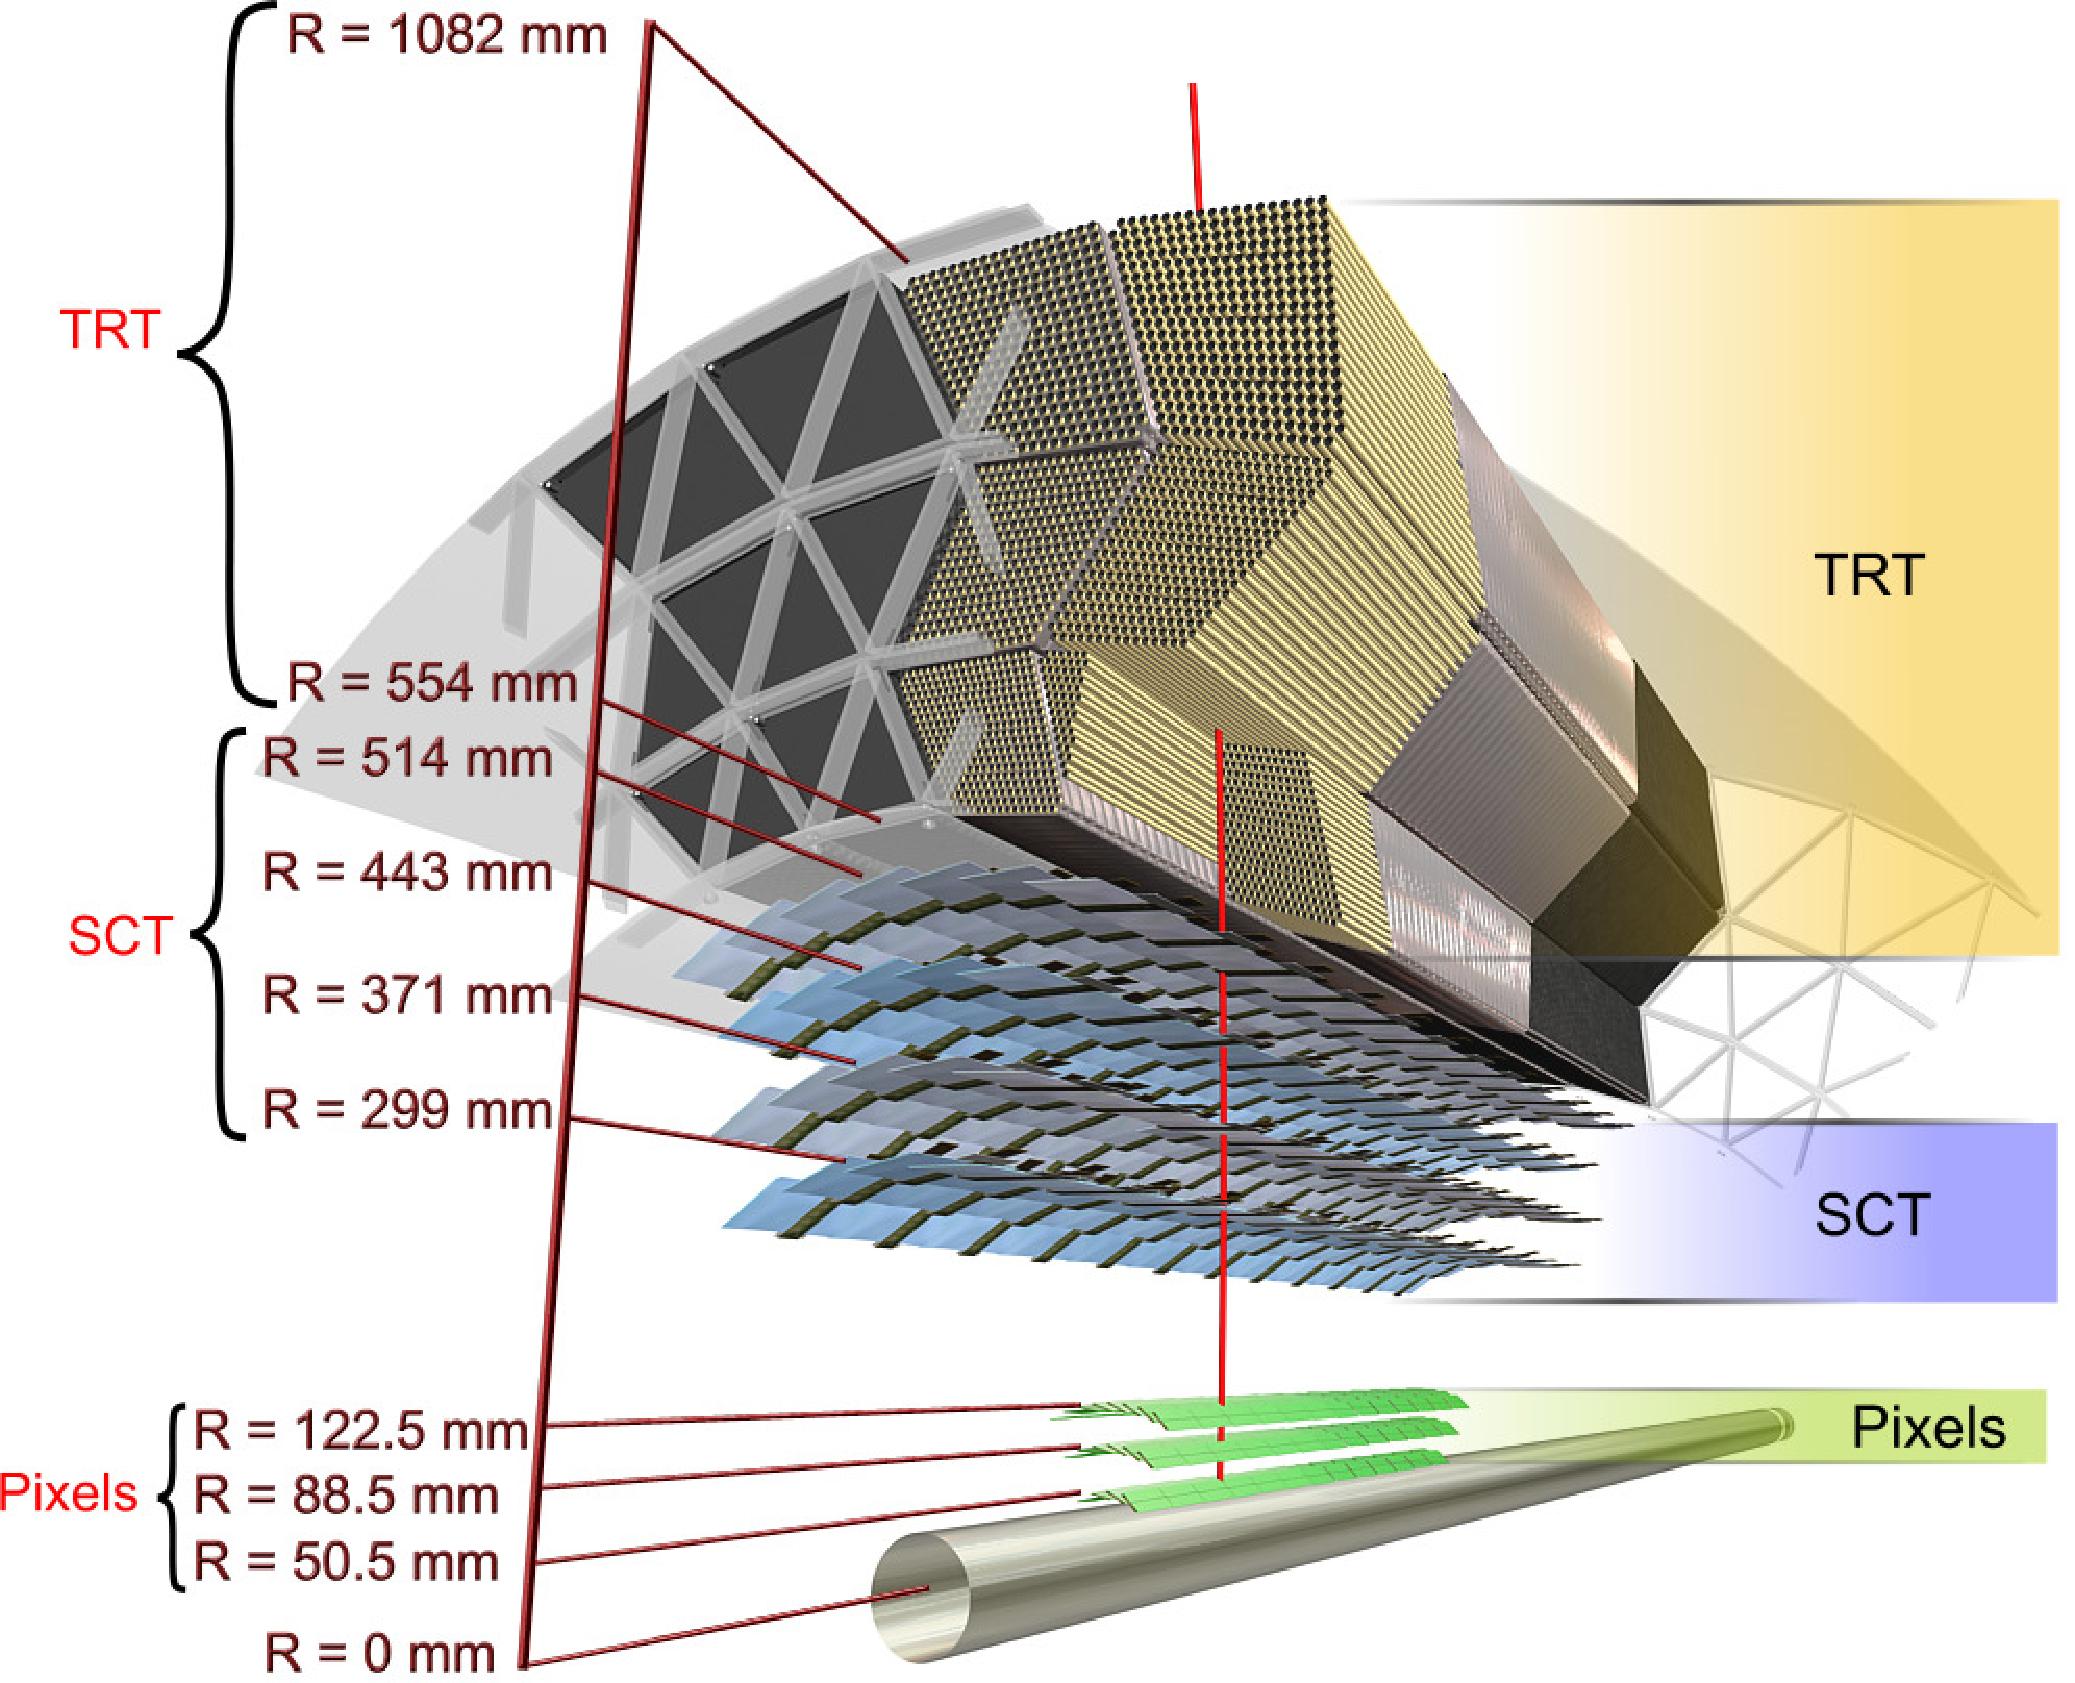
\includegraphics[width=0.9\textwidth]{figs/lhc/IDBarrel-eps-converted-to}
\caption{ Diagram of the ATLAS ID in the $R-\phi$ plane showing the barrel view of the Pixel Detector, SCT, and TRT.
}
\label{figure:lhc_id_barrel}
\end{figure}

\begin{figure}[!t]
\centering 
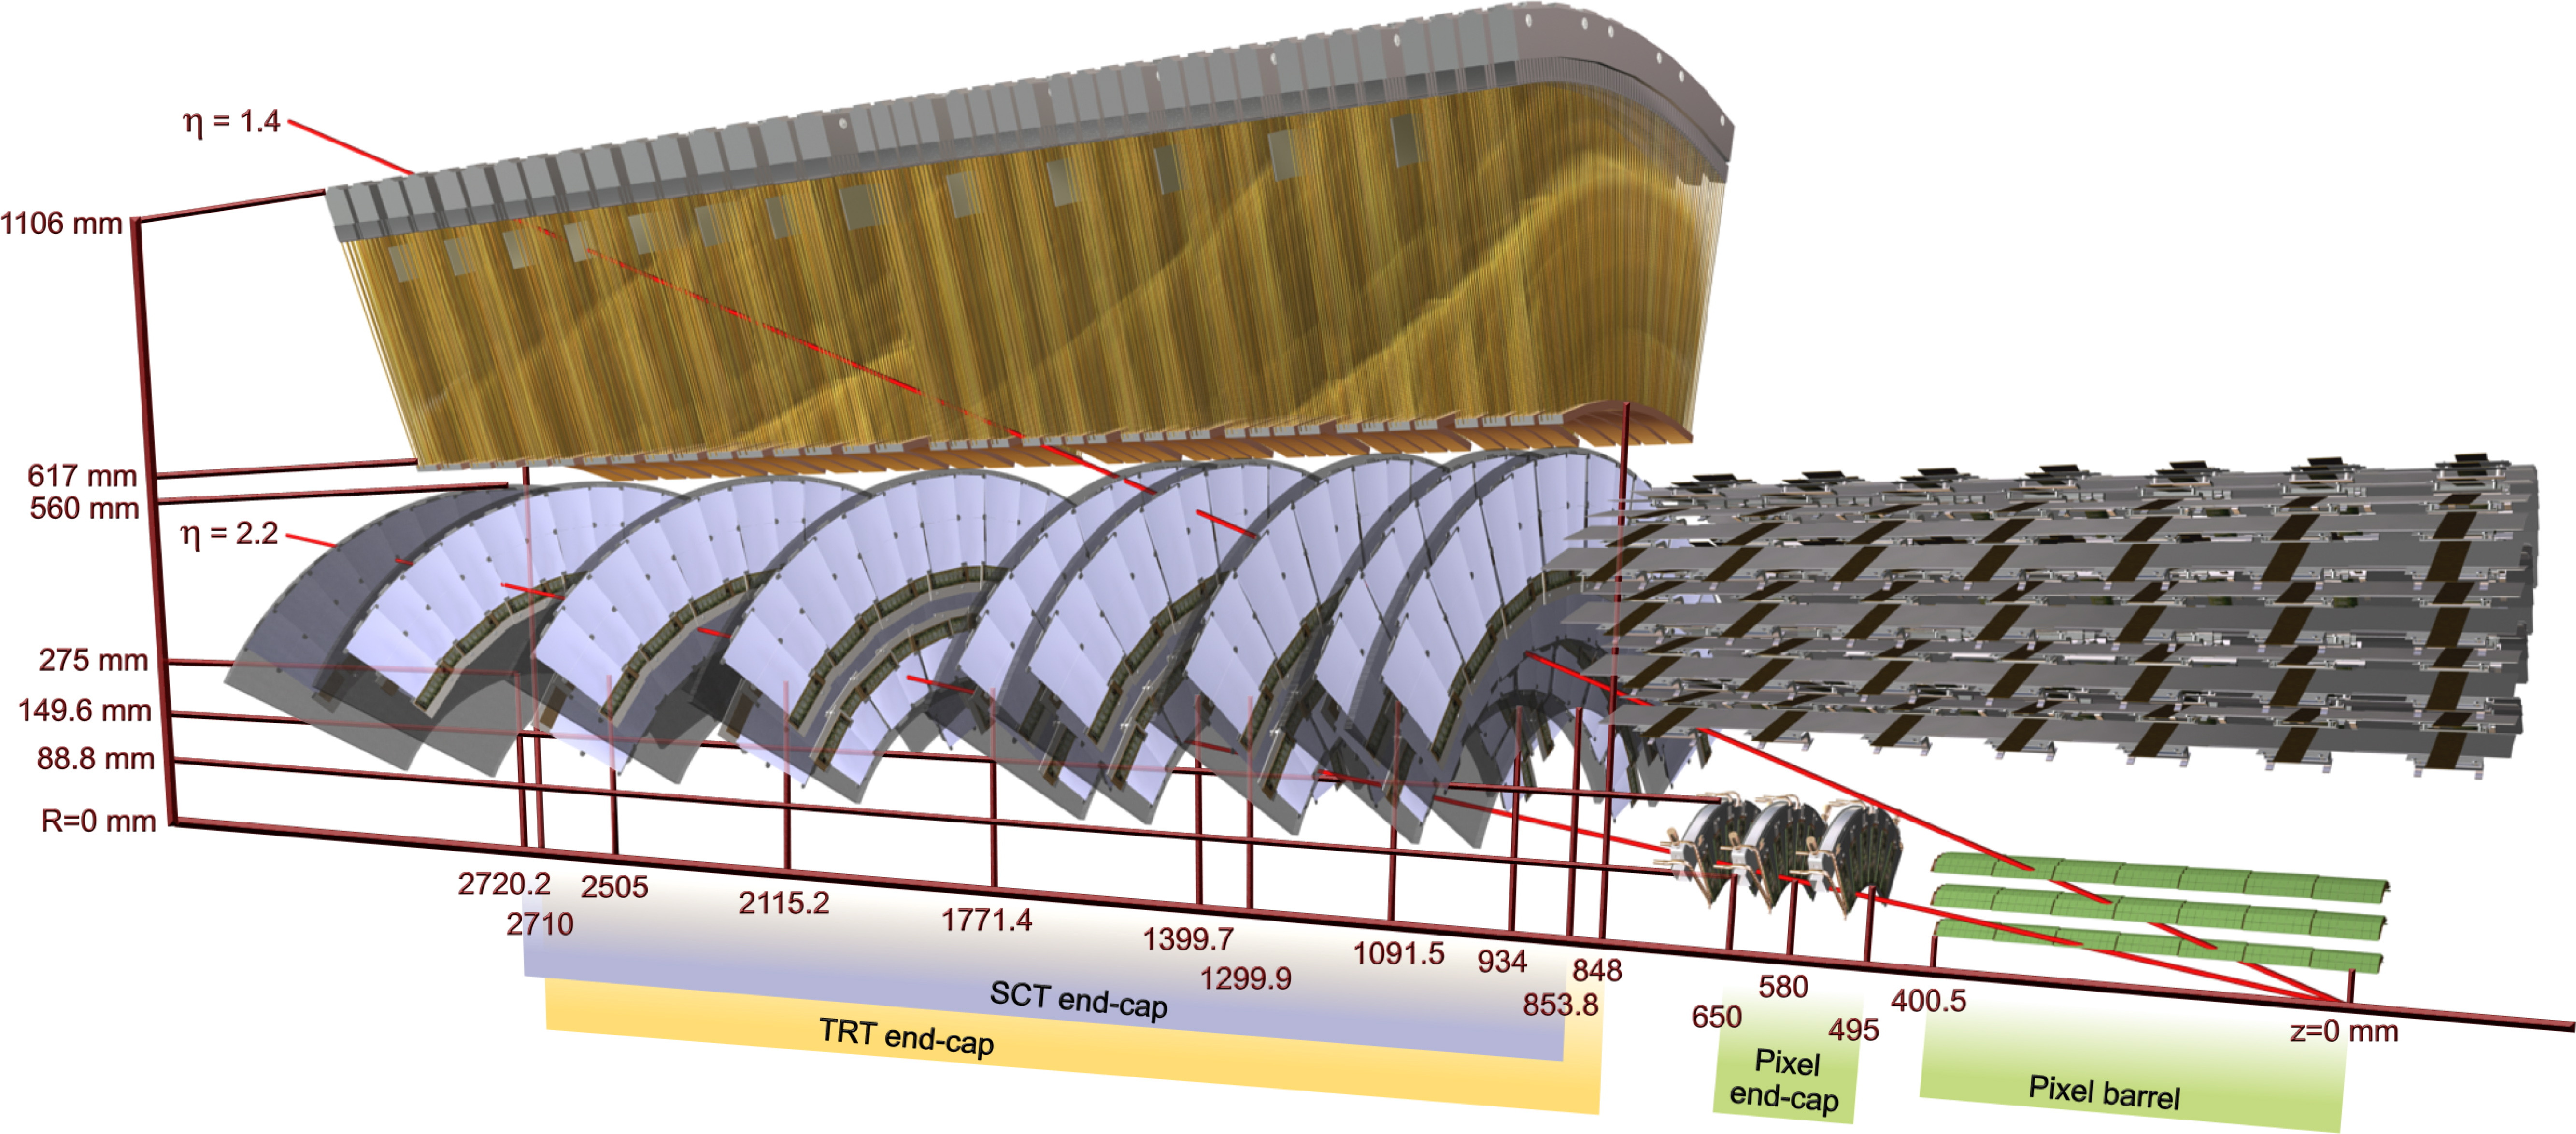
\includegraphics[width=0.9\textwidth]{figs/lhc/IDEndcap-eps-converted-to}
\caption{ Diagram of the ATLAS ID in the $R-z$ plane showing the endcap view of the Pixel Detector, SCT, and TRT. Only one side of the endcap is shown. 
}
\label{figure:lhc_id_endcap}
\end{figure}

The Pixel Detector has 80 million silicon read out channels (pixels) and is closest to the interaction point with the finest granularity. As charged particles traverse the silicon, they create electron-hole pairs, which are subsequently pulled apart in an electric field and can be captured and registered as a current pulse. The detector has three concentric layers of pixels in the barrel (to $|\eta| < 1.9$) and three endcap disks on each side of the barrel (to $|\eta| < 2.5$). The closest barrel layer to the beam pipe is called the b-layer. The pixels provide excellent hit resolution ($R-\phi$ accuracy of 10 $\mu$m and $z$\ ($R$) accuracy of 115 $\mu$m in the barrel (endcap)).

The SCT uses similar silicon technology to the pixels, but the each SCT layer contains a double layer of silicon strips, which are much longer in length than width. The SCT has 4 million read out channels and is arranged in 4 barrel layers and 9 endcap layers with coverage to $|\eta| < 2.5$. The double layers are inclined slightly with respect to each other so that these 1D sensors have 2D resolution for coincident hits. The resolutions are 580 $\mu$m in $z$\ ($R$) for the barrel (endcap) and 17 $\mu$m in $R-\phi$ .

The TRT is comprised of straw drift tubes filled with a gas mixture, containing mostly Xenon gas. Particles traversing the straws ionize the gas, and the liberated electrons drift to a wire at the center of the straw, which has an applied voltage, and induce an signal on the wire. The TRT has $\sim$300,000 straws. The barrel straws are arranged cylindrically along the $z$ direction out to $\sim|\eta| < 1$ and the endcap straws point radially outward in the $R$ direction. For this reason, the barrel (endcap) straws provide no measurement in the $R$\ ($z$) directions. The drift tubes provide individual position measurements with resolutions of $\sim$ 130 $\mu$m. Each particle track has on average 35 hits, which is large compared to the Pixel and SCT tracks, which have on average 7 hits. 

The TRT is unique in that it also provides particle identification measurements via transition radiation. Charged particles emit transition radiation when traversing a boundary between materials of different dielectric constants. The volume between the straws is filled with a radiator material, a polymer foil or foam, to provide this boundary condition. Transition radiation photons are emitted in the direction of the particle trajectory in the keV range and cause a much larger signal amplitude within the straw. Hits that cause a signal at a higher threshold are thus indicative of transition radiation.  The probability for emission transition radiation depends on the relativistic $\gamma$ of the traversing particle. Because electrons are much lighter than any other charged particle, their $\gamma$-factors tend to be high enough to induce transition radiations, as opposed to pions, muons and other particles. 

Combined tracking of particles through the 3 sub-detectors results in track momentum measurements from 500 MeV, the minimum energy need to leave the ID due to the magnetic field, to a few TeV. The track \pt\ resolution is roughly 0.05\%$\cdot$\pt\ $\oplus$ 1\%.  

\subsection{The Calorimeter}

The ATLAS calorimeters measure the energy of electrons, photons and hadrons with $|\eta|<4.5$. They induce a particle shower via electro-magnetic and nuclear interactions with the detector material and are deep enough to ensure that all or most of the shower energy remains contained. Exceptionally, muons pass through the ATLAS calorimeters leaving relatively little energy behind. ATLAS calorimeters are sampling calorimeters meaning that the active material of the detector only measures a small fraction of the energy produced by the shower. The overall shower energy is inferred from this fractional measurement. The rest of the material is inactive, dense material, designed to induce showers. The calorimetry system is grossly divided longitudinally (radially) into electro-magnetic (EM) and then hadronic segments, operated with different technologies. Figure~\ref{figure:lhc_calo} diagrams the layout of the calorimeter system.

\begin{figure}[!t]
\centering 
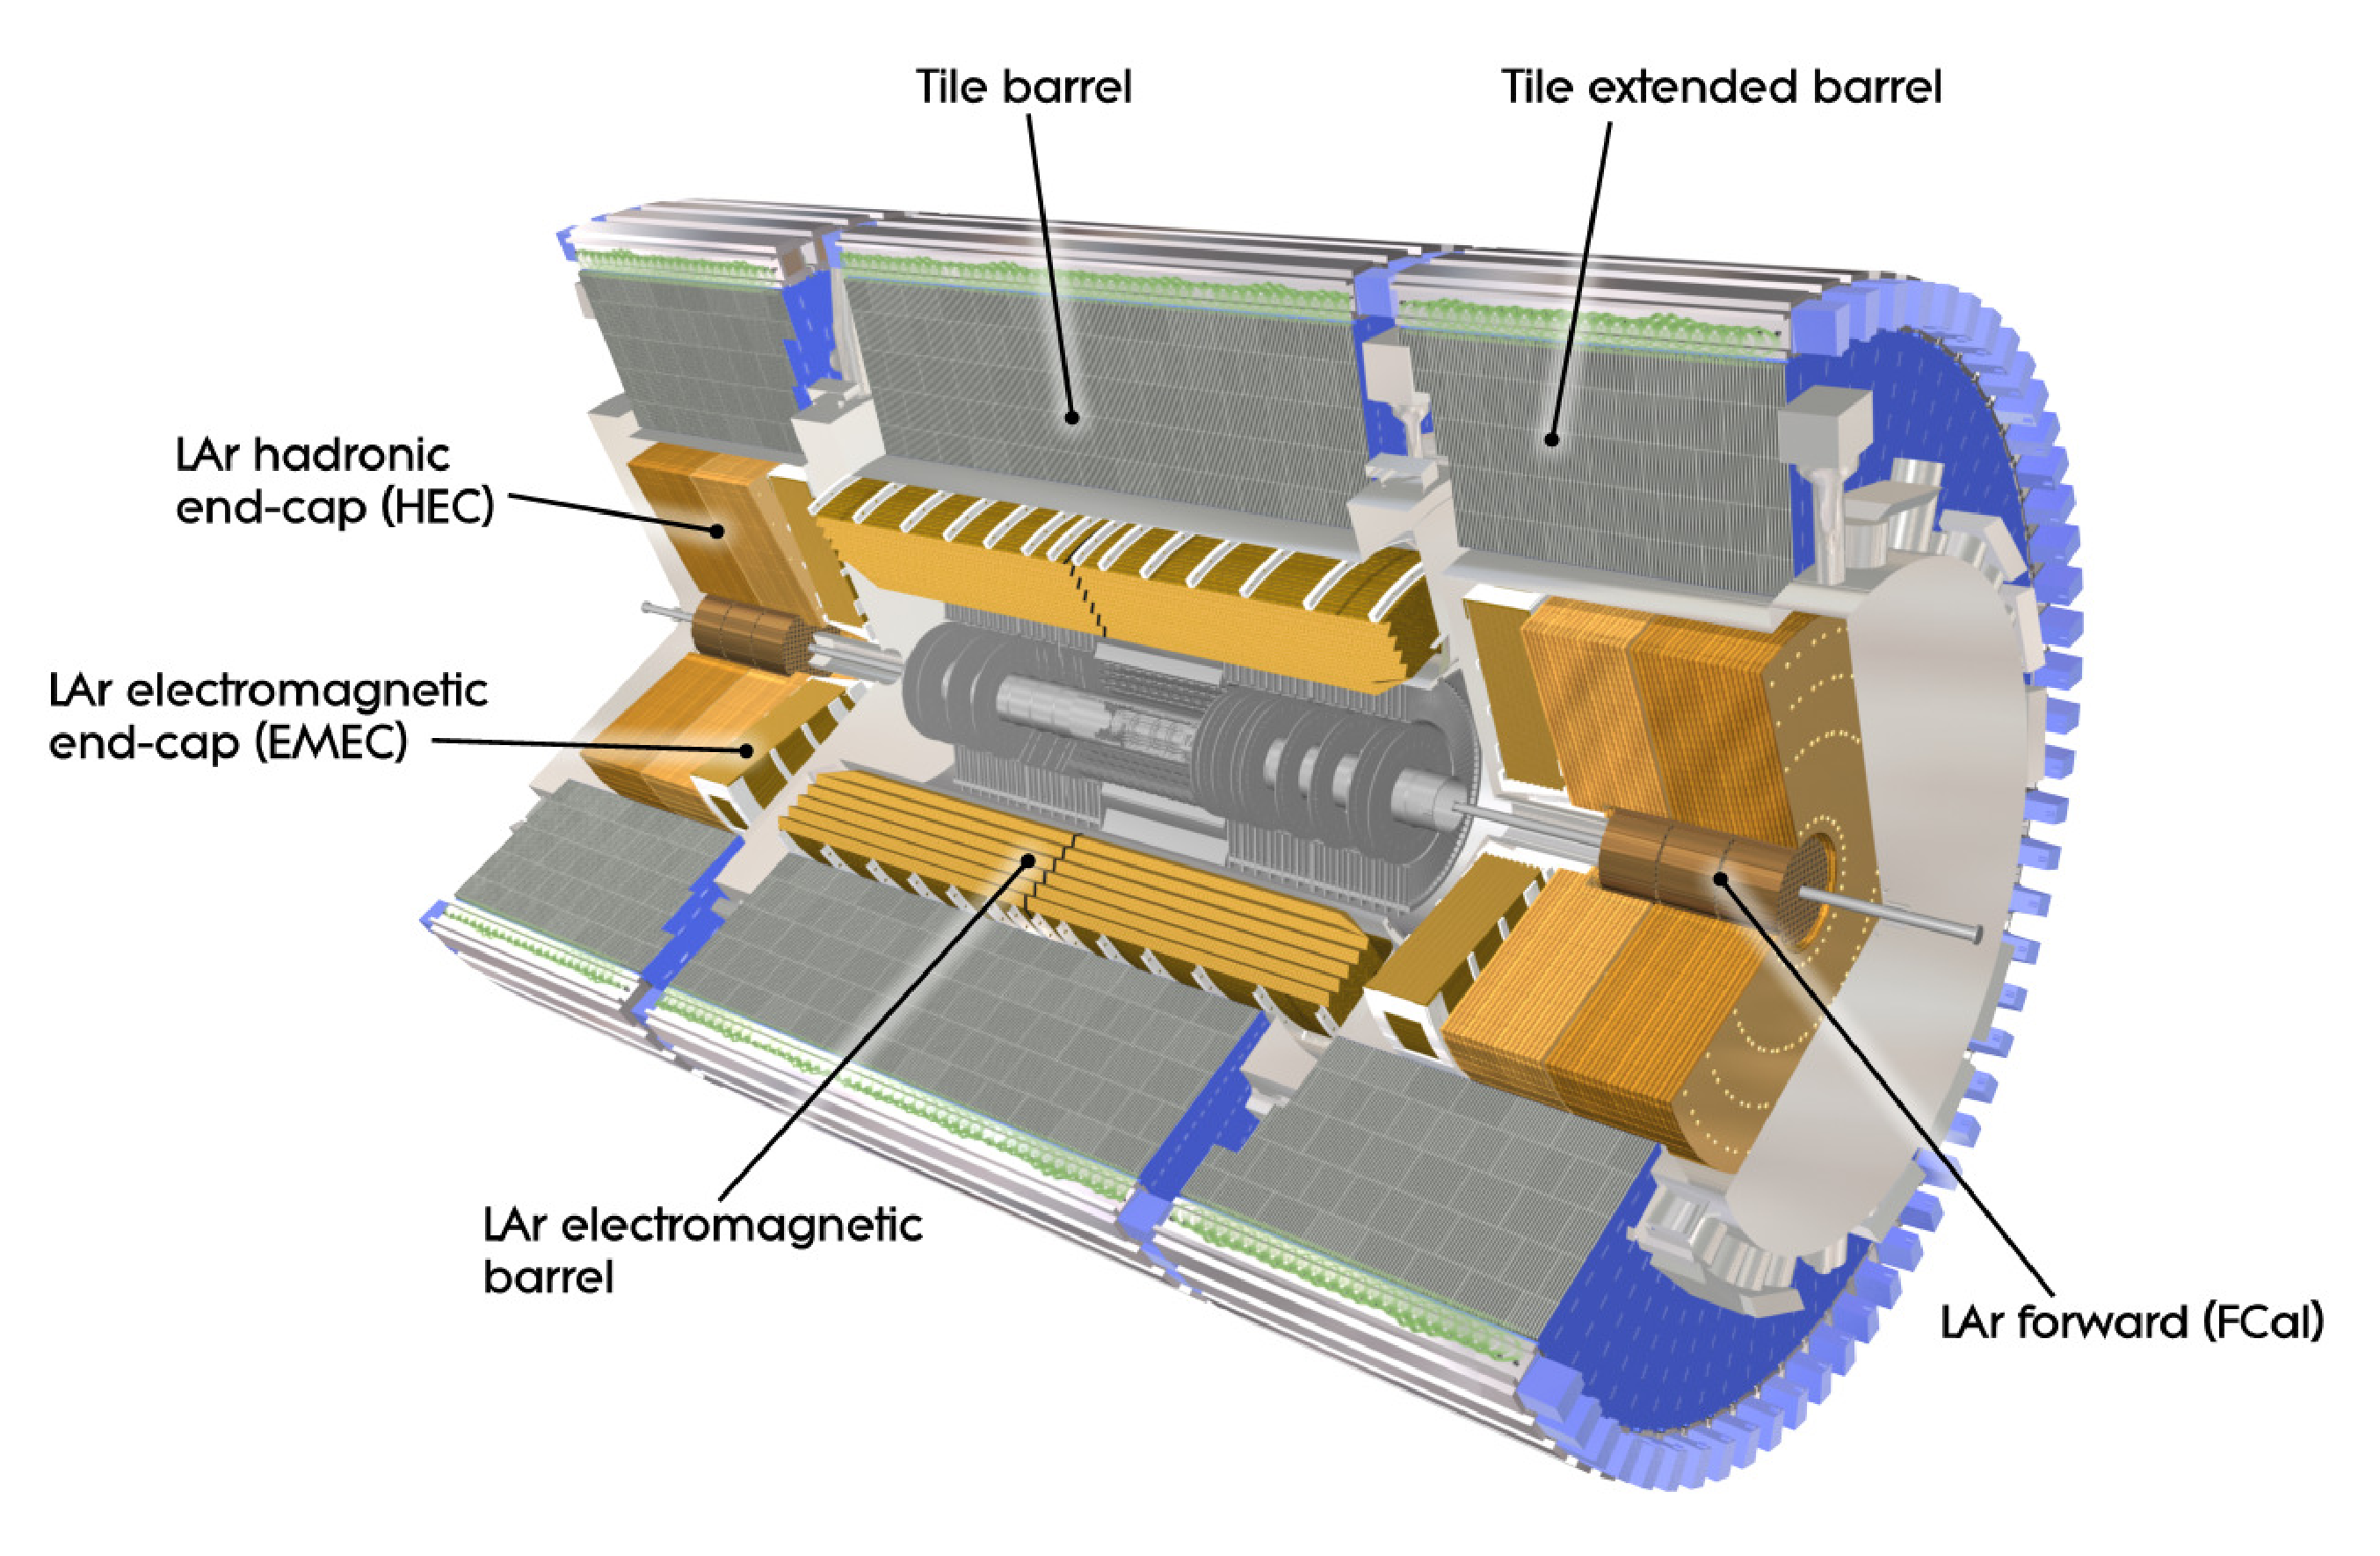
\includegraphics[width=0.9\textwidth]{figs/lhc/Calorimeter-eps-converted-to}
\caption{Diagram of the ATLAS calorimeters}
\label{figure:lhc_calo}
\end{figure}


The EM calorimeter (LAr), which is located directly outside of the solenoid magnet but within the same cryostat, has a accordion design with lead absorber and liquid argon active material. The accordion design ensures uniform coverage in $\phi$. The barrel and endcap LAr extend to $|\eta| < 2.47$. The LAr provides highly granular measurements in $\eta-\phi$ with 4 longitudinal segments, totaling $\sim$25-35 radiation lengths with the exception of the barrel/endcap transition region ($1.37<|\eta|<1.52$).  The geometry of the barrel LAr calorimeter can be seen in Figure~\ref{figure:lhc_calo_em}. The first longitudinal segment is called the pre-sampler, composed of a thin layer of active liquid argon, designed to detect early particle showers. The second segment is the most highly granular segment called the `strips', as it is composed of thin liquid argon cells. The strips have a size of $0.025/8$ x $0.1$ in $\eta-\phi$ in the barrel with similar sizes in the endcap and are designed to be able to resolve single and double particle showers. This resolution is particularly useful in distinguishing $\pi^0\rightarrow\gamma\gamma$ signatures from electron and photon signatures. The bulk of the radiation lengths and therefore the primary energy measurement come from the the third layer\footnote{this layer is actually called 'layer 2', since the pre-sampler is referred to as 'layer 0'}. Each cell in this layer is $0.025$ x $0.025$ in $\eta-\phi$. The final layer is coarser, thinner and designed to estimate energy leaking out of the EM calorimeter. The forward EM calorimeters extend the $\eta$ range and use the same technology, but are not used in this analysis. The energy resolution of the EM calorimeters is $\sigma_E/E = 10\%/\sqrt{E}\oplus0.7\%$, measured in test beam data and confirmed in collision data. 

\begin{figure}[!t]
\centering 
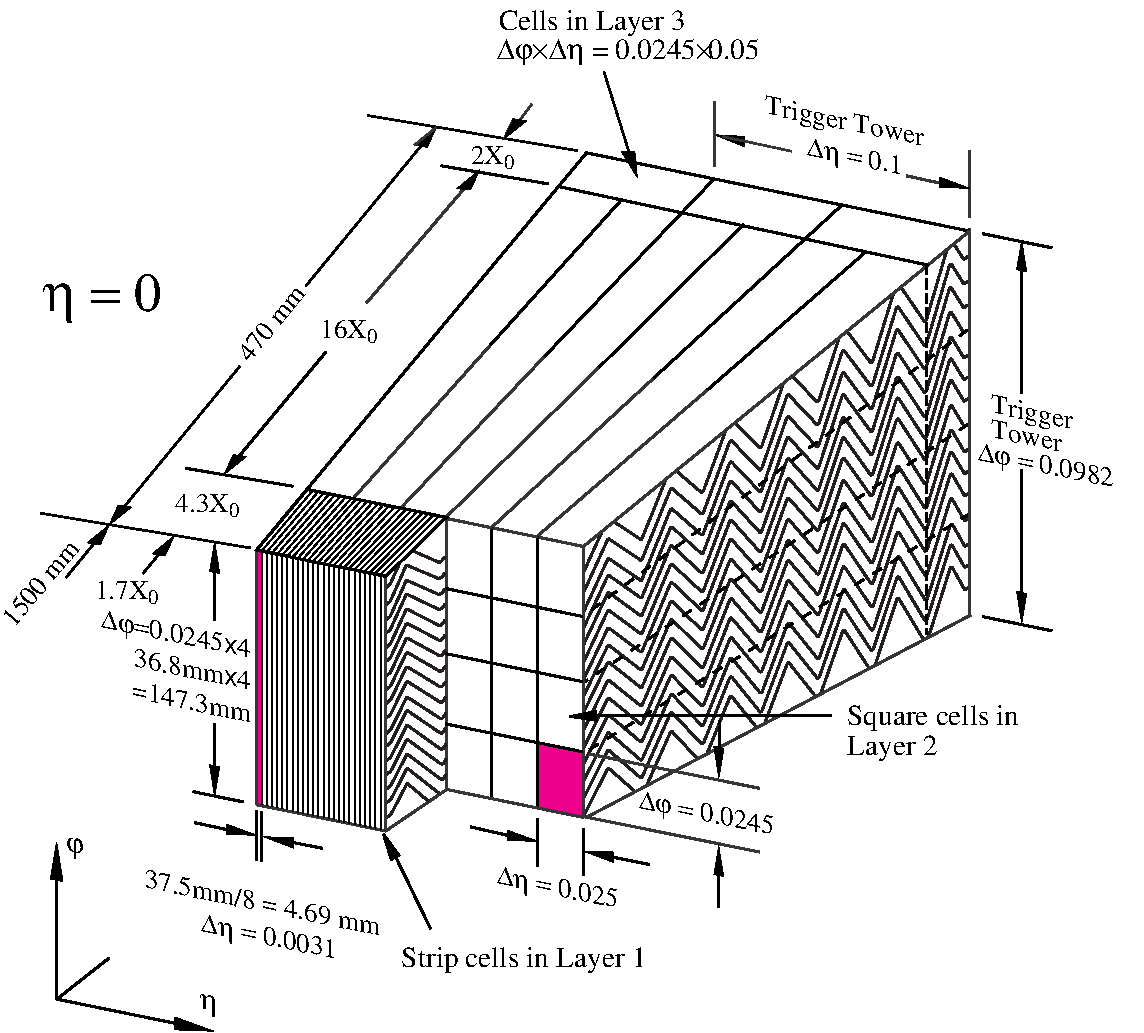
\includegraphics[width=0.9\textwidth]{figs/lhc/LARG3-TDR-barrelM-eps-converted-to}
\caption{Diagram of the ATLAS  LAr EM calorimeter showing the longitudinal segmentation and the $\eta-\phi$ cells for the central barrel region}
\label{figure:lhc_calo_em}
\end{figure}




The hadronic calorimeter is located directly behind the EM calorimeter. It is composed of tiles of iron absorber and plastic scintillator  in the barrel ($|\eta| < 1.6$), called the TileCal,  and copper-liquid argon in the endcap ($1.5<|\eta| <3.2$), called the HEC. The calorimeters contain $\sim$10-19 hadronic interactions lengths with multiple longitudinal segments to contain showers induced by the nuclear interaction of hadronic particles. The energy resolution of the hadronic calorimeters is $\sigma_E/E = 50\%/\sqrt{E}\oplus3\%$. The intrinsic resolution of hadron calorimeters is much worse than electro-magnetic calorimeters, because much of the energy is lost to the inelasticity of nuclear break-up. 

\subsection{The Muon Spectrometer} 

The MS measures the trajectory of particles outside of the calorimeters, using multiple different technologies. Generally, all charged particles except for muons are stopped by the calorimeter, and therefore the majority of particles in the MS are muons, with the exception of rare cases of hadronic punch-through. Particle momentum spectroscopy is made possible by an air-core toroidal magnet system, embedded in the barrel MS ($|\eta| < 1.4$), and two smaller end cap toroids that provide fields out to $|\eta| < 2.7$. 

In the barrel region, the muon chambers are arranged in three cylindrical layers around the beam, while in the endcap-regions the layers are arranged perpendicular to the beam in wheels. The arrangement is depicted in Figure \ref{figure:lhc_muon}.

\begin{figure}
\centering 
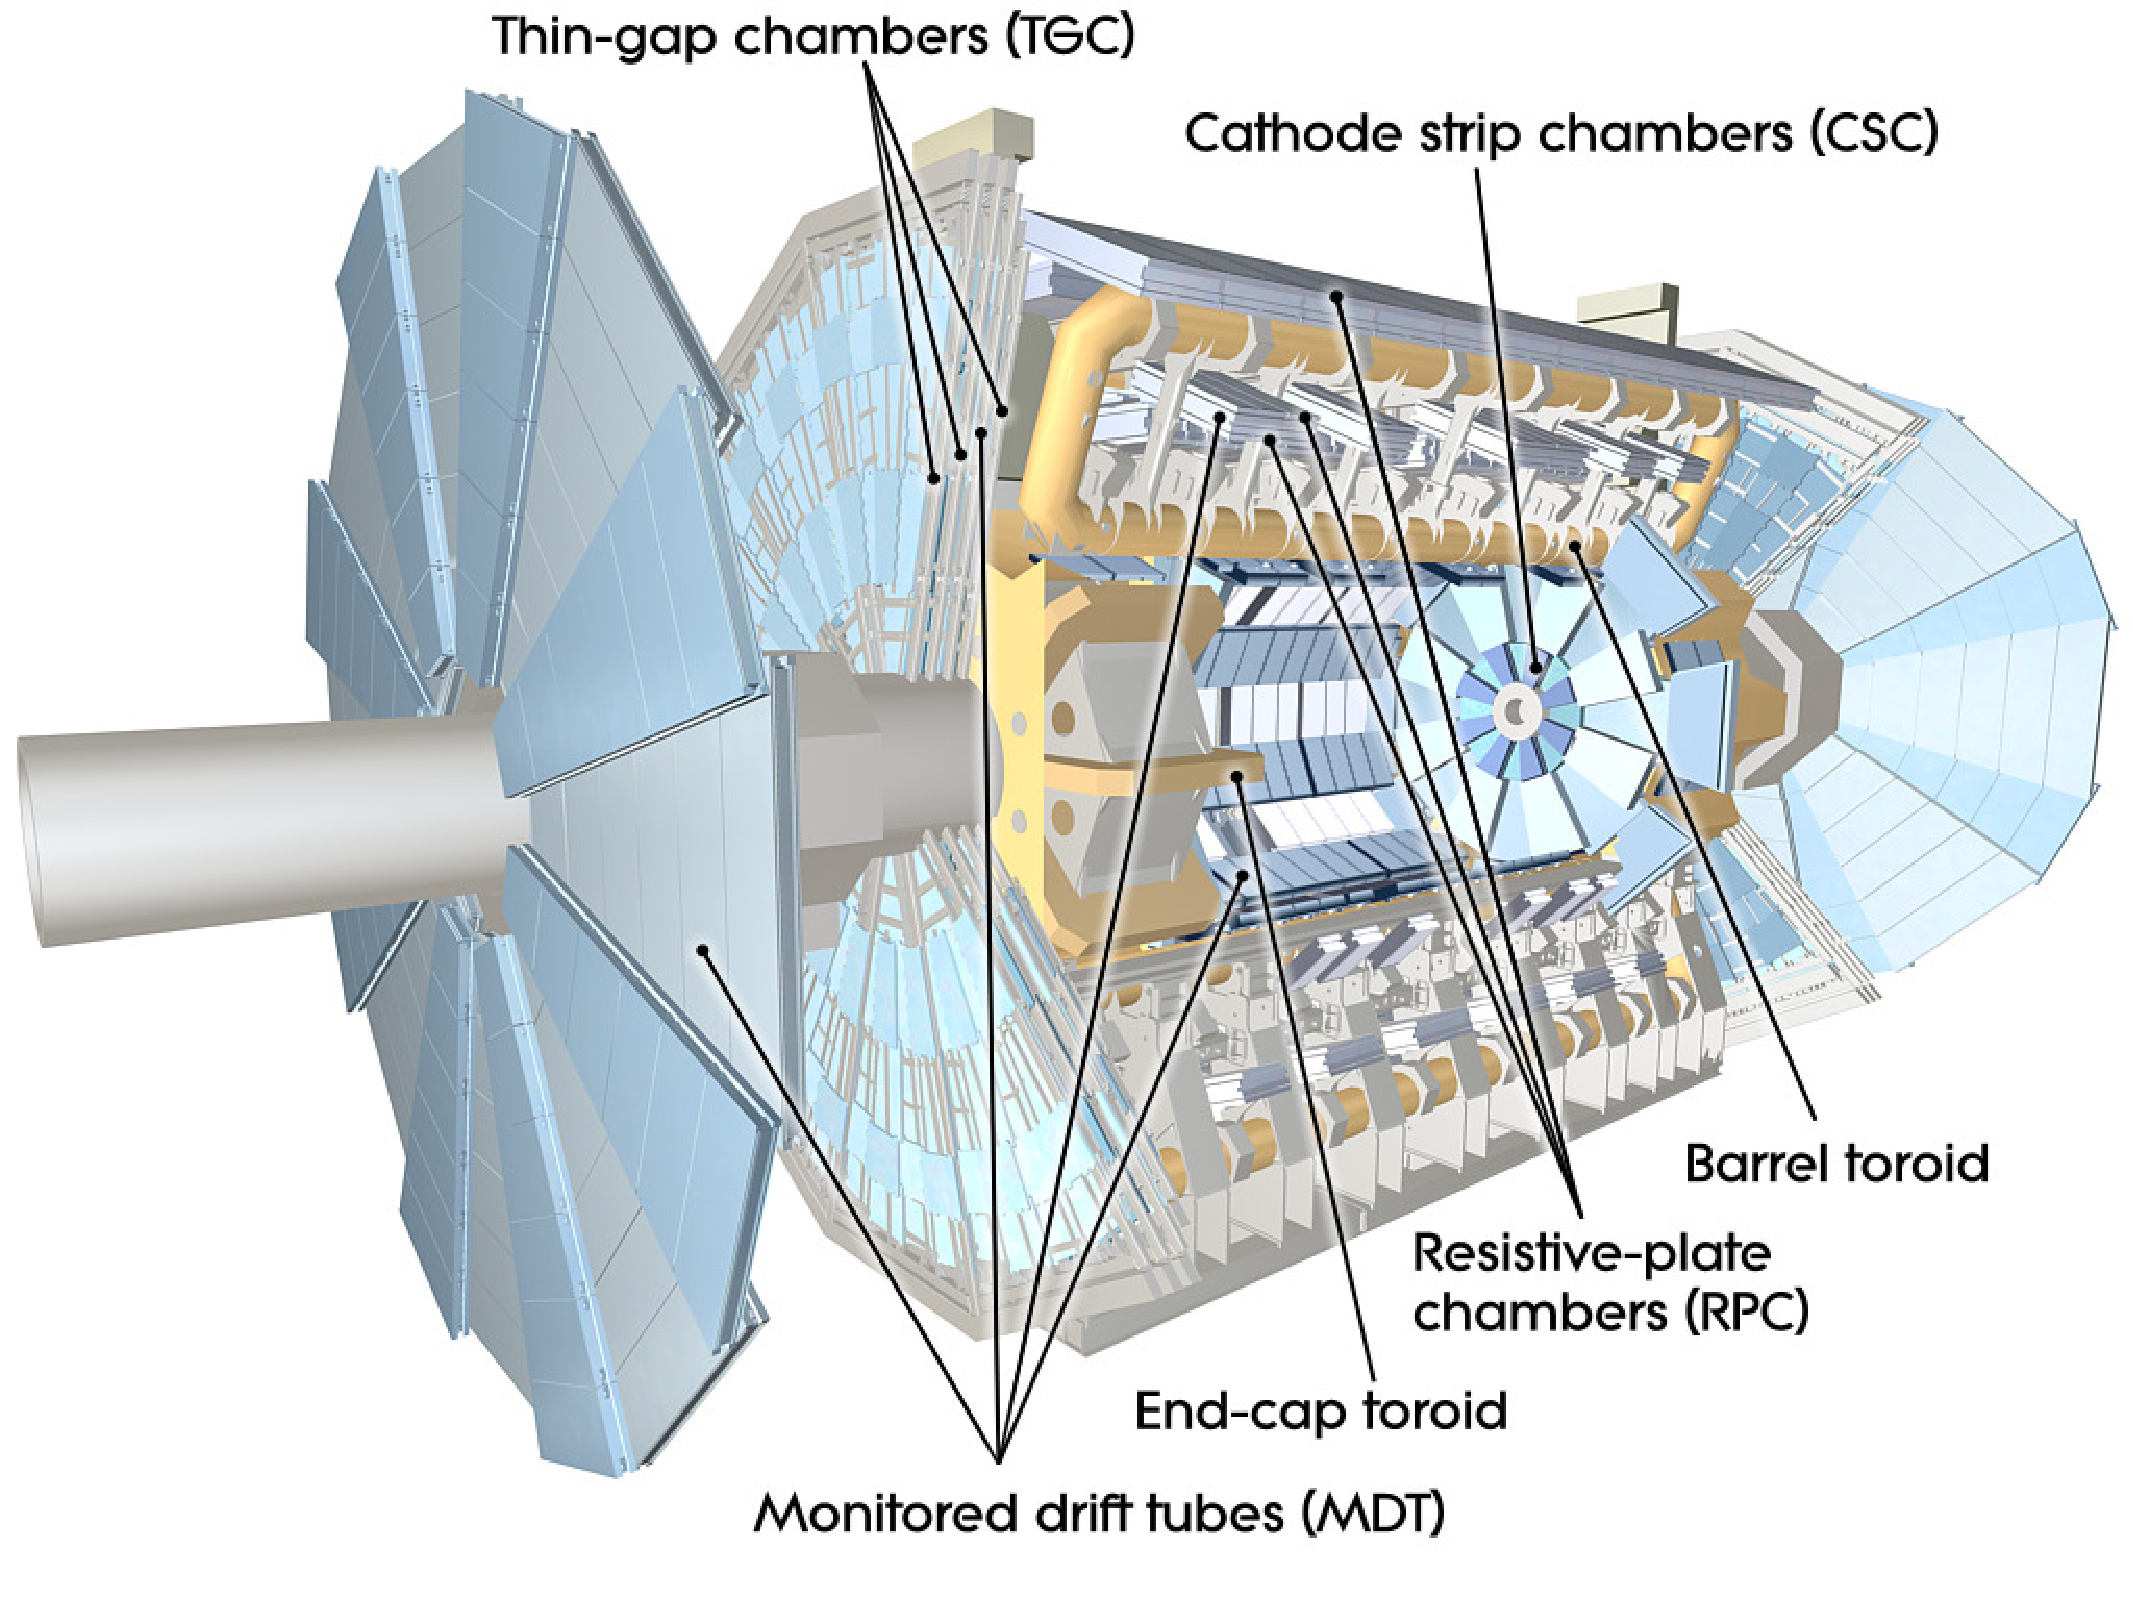
\includegraphics[width=0.9\textwidth]{figs/lhc/MuonSystem-eps-converted-to}
\caption{Diagram of the ATLAS muon system}
\label{figure:lhc_muon}
\end{figure}

The chambers in the barrel and most of the endcap are constructed from Monitored Drift Tubes (MDTs) with an Argon gas mixture. Each chamber contains 3-7 drift tubes and provide hit resolutions of 80 $\mu$m per tube and 35 $\mu$m per chamber in the bending plane. For $|\eta| > 2.0$, Cathode Strip Chambers (CSCs) are used, primarily to handle the higher incident particle flux. They are composed of cathode strips crossed with anode wires in the gas mixture, but use similar drift technology as the MDTs and have resolutions in the bending plane 40 $\mu$m per chamber. 

Separate chambers, called Thin Gap Chambers (TGCs), used in the endcaps, and Resistive Plate Chambers (RPCs), used in the barrel, provide less precise hit information but within a much quicker time window, and are therefore used for triggering, as the CSCs and MDTs are too slow.


\subsection{The Trigger System} 


The ATLAS trigger system is designed to make quick decisions about individual particle collisions to reduce the enormous collision rate of 20 MHz to a much more manageable 400 Hz to be stored for offline analysis. Saving the full ATLAS data-stream would require space for 40 TB of raw data per second, but, more importantly, most of these collisions result in the uninteresting inelastic break-up of the colliding protons. To select out collisions to allow for a diverse physics program, ATLAS devotes a large portion of the bandwidth to general purpose single lepton triggers ($\sim$ 250 Hz). The presence of leptons in the event indicates the presence of the weak or electro-magnetic interaction and therefore occurs at many order of magnitude less frequently then interactions involving the strong interaction. Moreover, many interesting physics signatures that are analyzable by ATLAS involve leptonic final states. The remaining bandwidth is allocated to jet, missing energy, tau, and unbiased supporting triggers.

The ATLAS trigger system is composed of 3 levels: level-1 (L1), level (L2), and the event filter (EF). The first level is a hardware only trigger that reduces the input 20 MHz rate to $\sim$ 75 kHz, selecting 1 out of every 250 collisions. The available buffering on the chips means that the decisions need to be made within 2.5 $\mu$s. The L1 identifies small areas of the detector with significant energy, called Regions-of-Interest (ROIs).

The second and third stages L2 and EF are software based. The L2 algorithms perform more detailed object reconstruction for leptons, jets and photons inside of the ROIs provided by L1, by performing tracking and in depth calorimeter clustering algorithms. The decisions are made within 50 ms per event and pass 1 out of every 15 events to the EF. At the EF, events undergo full reconstruction using similar but faster versions of the algorithms used offline. The EF makes decisions on the presence of fully identified objects in the event and event topological quantities within 4s to reduce the L2 output by a factor of 10. The events that pass this stage are then written to tape for offline study.



\subsection{Reconstruction: Jets, Muons and Electrons}

Physicists analyze the collision event as a collection of identified objects, expressed as particles' momentum 3-vectors. The process of converting the disparate detector signatures and signals into a unified 4-momentum description of individual objects is called reconstruction. These objects arise from the final state particles in the event, which can be combined and counted to infer properties of the hard scatter. The particles that make detectable signatures are muons, electrons, photons, and jets of hadrons. Jets and b-tagged jets, muons and electrons are used in the \tth\ analysis to define our search regions and to separate the Higgs signal from backgrounds. Other analyses use photons, taus and missing transverse energy\footnote{missing transverse energy is the presence of momentum imbalance in the transverse plane of the calorimeter due to escaping neutrinos}, but these are not discussed in depth here. Figure~\ref{figure:lhc_particles} shows an $R-\phi$ schematic of the interaction of various particle signatures in the ATLAS detector.  

 

\subsubsection{Tracks and Clusters}

The basic components of reconstruction are sensor measurements, or hits, in trackers (ID, MS) and energy measurements in the calorimeter. Hits in the ID and MS undergo pattern recognition, which identifies hits that belong to a single track, and fitting, which fits a curve to the track to assess the particle trajectory. Charged particle trajectories are generally helical in a magnetic field, but the fitting algorithm takes into more detailed information about energy loss to material along the tracks length. The result of the fitting is an estimation of particle momentum 3-vector. Electrons, photons and hadronic particles leave clustered deposits of energy in the EM and hadronic calorimeters from their showers. Electron and photon showers are primarily contained with the EM calorimeter, while hadronic showers deposit most of their energy in the hadronic calorimeters. The process of associating individual read-out cells of energy in the calorimeter to clusters of energy from the showers of individual particles is called clustering. From the basic pieces of tracks and clusters, more complex objects can be created. 

\subsubsection{Electrons}

Electrons leave both a track in the ID and a narrow and isolated cluster of energy in the EM calorimeter, $\Delta R < 0.1$. Electron reconstruction proceeds using a sliding window algorithm, which scans a fixed size rectangle in $\eta-\phi$ space over the EM calorimeter cells to find relative maxima of energy in the window \cite{ATLAS-CONF-2014-032}. These maxima seed the clustering algorithms. Because electrons are light, they lose energy to the material gradually through scattering and more catastrophically through the emission of a high energy photon, through interaction with nuclei. This process is called bremsstrahlung. Tracks for electrons are reconstructed differently because they must include the hypothesis that the electron loses significant energy through bremsstrahlung. Generally, the emitted photon is contained within the same energy cluster and therefore the sliding window algorithm is always wider in the direction of bending, $\phi$. A single track is then matched to the cluster within certain minimum matching requirements in $\eta$, $\phi$, and \pt. Electrons are distinguished from photon conversions, which also have a track, by lack of association with conversion vertices, found with a dedicated algorithm.

Electrons have many lever arms for further identification to suppress backgrounds from fake sources. The narrowness of the shower shape, quality of track, and presence of transition radiation are used by cut-based and multivariate identification algorithms. This is discussed in depth in Chapter \ref{chapter:electron}. Electrons are reliably reconstructed and identified with energies above 7 GeV. 

\subsubsection{Muons}

Muons are reconstructed from a combination of ID and MS tracks, when possible. The two tracks must meet matching criteria to ensure they are from the same particle. The muon momentum 3-vector comes from the combined ID/MS fit. Muons leave little energy in the calorimeters and are generally isolated from other particles, when produced from electro-weak bosons. Identification algorithms make requirements on the number of tracking hits in the ID and MS and the quality of the matching of the two tracks. Muons are reliably reconstructed and identified with energies above 5 GeV. More about muon reconstruction and identification can be found here~\cite{MCP2012}.


\subsubsection{Jets}

Quarks and gluons are colored objects that cannot exist alone on the time scales of detector measurements, due to confinement, a property of the strong force . When emitted, they undergo a process called hadronization, in which they convert into `jets' of colorless hadrons that emerge collimated from the interaction point. The majority of these hadrons are charged and neutral pions, though other hadrons are often present. Jets are reconstructed using conglomerations of calorimeter energy clusters chosen via an anti-k$_t$ algorithm, with a radius of $\Delta R <$0.4 ~\cite{Cacciari:2008gp}. The algorithm has been shown to be infrared safe, meaning the jet quantities are not sensitive to low energy, small angle radiative divergences. Jets at ATLAS are reconstructed from 10 GeV, calibration of the energy scale and resolution are only available for energies greater than 20-25 GeV. 

\subsubsection{B-Tagged Jets}
Generally, the flavor of the initiating quark is not known from the reconstructed jet, although gluon initiated jets and quark initiated jets have slightly different properties. Jets from b quarks, however, are unique in that the long life-time of the produced B mesons allow for measurable decays in flight. This property is used to tag b-quark initiated jets. This analysis uses the MV1 tagging algorithm \cite{ATLAS-CONF-2011-102}, which is a neural network based algorithm that looks for secondary displaced decay vertices inside the event and takes into account jet track parameters and energy flow with respect to these vertices. Jets from b quarks often involve B meson decays to leptons, especially muons, which can be used to tag an orthogonal b-jet sample for studying tagging efficiencies.

\begin{figure}
\centering 
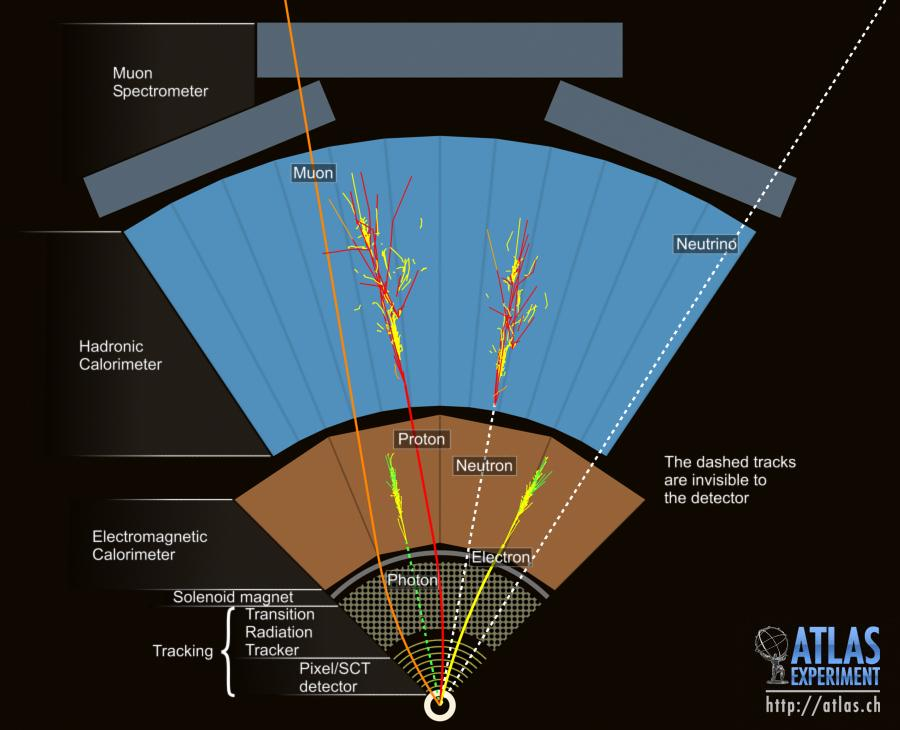
\includegraphics[width=0.9\textwidth]{figs/lhc/particles.jpeg}
\caption{$R-\phi$ schematic of the ATLAS detector and various particle signatures}
\label{figure:lhc_particles}
\end{figure}

